
% ==============================================================================
\section*{Introducción}
% ==============================================================================


Un sistema de distribución eléctrica es la porción de la infraestructura de suministro de energía que toma la electricidad de los circuitos de transmisión de alta tensión y la entrega a los clientes. Este sistema se estructura típicamente en niveles jerárquicos de voltaje.

\subsection*{Media Tensión (MT)}
Generalmente, los circuitos de distribución primaria se consideran de \textbf{"media tensión"} (medium-voltage), abarcando normalmente desde $600 \text{ V}$ hasta $35 \text{ kV}$. Las líneas de distribución primaria (alimentadores) operan típicamente entre $2.2 \text{ kV}$ y $34.5 \text{ kV}$. Estos circuitos distribuyen la energía desde las subestaciones hacia las áreas de consumo.

\subsection*{Baja Tensión (BT)}
Cerca de cada usuario final, un transformador de distribución reduce el voltaje de la distribución primaria a un circuito secundario de \textbf{bajo voltaje} (low-voltage secondary circuit). Las tensiones de utilización comunes en América del Norte son $120/240 \text{ V}$. Los sistemas de distribución secundaria están diseñados para mover la energía solo unas pocas cientos de yardas de manera eficiente, lo que restringe la ubicación de los transformadores de servicio.

\subsection*{Importancia del Sistema de Distribución}
El sistema de distribución es fundamental por varias razones:
\begin{enumerate}
    \item \textbf{Fiabilidad y Calidad del Servicio}: Es a menudo el componente más crítico en términos de su efecto en la fiabilidad (\textit{reliability}) y la calidad del servicio. El rendimiento del sistema de distribución determina más del $90\%$ de la fiabilidad del servicio a los clientes.
    \item \textbf{Entrega Universal}: Los sistemas de distribución entregan electricidad literalmente en todas partes, a clientes concentrados en ciudades, en los suburbios y en regiones muy remotas.
    \item \textbf{Seguridad}: La seguridad es una consideración muy importante en el diseño, operación y mantenimiento de las instalaciones de distribución, incluyendo aspectos como la protección contra rayos y la puesta a tierra.
\end{enumerate}


% ==============================================================================
\section*{Desarrollo}
% ==============================================================================

\subsection*{Herrajes (\textit{Hardware})}
Los herrajes (conectores y accesorios) son a menudo los eslabones débiles en el sistema aéreo, debido a ambientes hostiles, malos diseños o, más comúnmente, a una instalación deficiente.

\begin{enumerate}
    \item \textbf{Abrazadera de suspensión}: Las líneas aéreas utilizan construcciones de suspensión. Las estructuras aéreas requieren herrajes con suficiente resistencia mecánica para soportar el peso de los conductores, el hielo acumulado y resistir la presión del viento.

    % Si está usando la clase apa7, el comando \figurenote{} es el recomendado.


    \item \textbf{Grapa de retención}: Están relacionadas con los conectores y empalmes. Los empalmes automáticos están disponibles para conductores bajo tensión, donde abrazaderas dentadas dentro del empalme sujetan el conductor.
    \item \textbf{Pernos} (de anclaje y de suspensión): Los pernos pasantes (\textit{through bolts}) se utilizan en construcciones de doble brazo (\textit{double-arming}).
    \item \textbf{Tornillos de seguridad}: Las fuentes mencionan el uso general de herrajes, pero no se proporciona una descripción específica o el uso de "tornillos de seguridad" con esa terminología.
    \item \textbf{Pasadores y arandelas de seguridad}: Los aisladores son a menudo del tipo de perno (\textit{pin type}). Añadir una arandela de aluminio o cobre sobre el brazo horizontal (\textit{crossarm}) bajo la brida del perno de acero puede reducir la rotura del aislador por choque térmico.
    \item \textbf{Conector de compresión}: La mayoría de los conectores primarios utilizan algún tipo de compresión para unir conductores. Utilizan matrices y herramientas para apretar dos conductores y el conector.
    \item \textbf{Mordaza de conexión a tierra}: Los herrajes de puesta a tierra incluyen cables de bajada conectados al neutro \textit{multigrounded} y deben poder manejar la corriente de falla total.
    \item \textbf{Separadores para conductores}: Los cables espaciadores (\textit{spacer cables}) son una configuración empaquetada que utiliza un cable mensajero para sujetar tres conductores de fase con cable cubierto.
    \item \textbf{Guardacables}: Implícito en las cubiertas de protección. Los protectores de bujes y los cables cubiertos son métodos muy buenos para reducir las interrupciones causadas por animales.
    \item \textbf{Aislador de perno}: Los aisladores se clasifican como de tipo \textit{pin} (perno), tipo poste o de suspensión.
\end{enumerate}

\subsection*{Postes}
Los postes son elementos estructurales cruciales para la construcción de líneas aéreas. Las líneas de distribución aéreas utilizan postes, normalmente de $30 \text{ a } 45$ pies de altura, instalados de $6 \text{ a } 8$ pies de profundidad.

\subsubsection*{Comparación de materiales}
\begin{itemize}
    \item \textbf{Madera} (\textit{Wood}): Es el principal material utilizado. La madera tratada dura mucho tiempo, es fácil de escalar y aumenta el aislamiento. Los postes de madera pueden pudrirse.
    \item \textbf{Acero} (\textit{Steel}): Las estructuras de acero y concreto reducen considerablemente el nivel de aislamiento (\textit{Critical Flashover Voltage, CFO}).
    \item \textbf{Concreto} (\textit{Concrete}): Al igual que con el acero, el uso de estructuras de concreto reduce significativamente el CFO.
    \item \textbf{Fibra de Vidrio} (\textit{Fiberglass}): También se utiliza fibra de vidrio. Las abrazaderas de aisladores de fibra de vidrio se utilizan en construcciones sin crucetas (\textit{armless constructions}).
\end{itemize}

\subsection*{Aisladores}
Los aisladores se utilizan para evitar fugas de voltaje y el contacto con tierra.

\subsubsection*{Clasificación y Tipos}
Los aisladores utilizados en líneas aéreas son de tipo \textit{pin} (perno), tipo poste o de suspensión.
\begin{itemize}
    \item \textbf{Aisladores Tipo Pin} (\textit{Pin Type}): Se montan en pernos o pasadores.
    \item \textbf{Aisladores de Suspensión} (\textit{Suspension Type}): Se utilizan en líneas aéreas.
    \item \textbf{Aisladores Tipo Poste} (\textit{Post Type}): Pueden usarse en construcciones sin cruceta.
\end{itemize}

\subsubsection*{Comparación de Materiales}
\begin{itemize}
    \item \textbf{Porcelana} (\textit{Cerámica}): Históricamente comunes. Los arcos eléctricos pueden dañarlos. Una falla interna en una carcasa de porcelana puede explotar y expulsar la porcelana como metralla.
    \item \textbf{Vidrio} (\textit{Glass}): Las fuentes no describen explícitamente su uso principal en distribución.
    \item \textbf{Polímeros} (\textit{Composite/Polymer}): Alternativa a la porcelana. Tienen un rendimiento superior para los arcos superficiales. Su principal ventaja es un modo de falla más seguro.
\end{itemize}

\subsection*{DPS y Protecciones}

\subsubsection*{DPS (Dispositivos de Protección contra Sobretensiones / \textit{Surge Protective Devices})}
Se refieren a los descargadores de sobretensión (\textit{surge arresters}), cuya función es la protección contra los rayos y las sobretensiones.

\textbf{Principio de Funcionamiento y Función}: Los descargadores de sobretensión (DS) de \textbf{óxido metálico} (\textit{Metal-Oxide Surge Arresters, MOV}) son tan no lineales que no requieren un espacio de aire (\textit{gap}). Bajo condiciones normales, el DS es un circuito abierto, pero cuando se dispara, se convierte virtualmente en un cortocircuito.

\subsubsection*{Protecciones (\textit{Protective Equipment})}
La protección contra cortocircuitos o sobrecorriente es muy importante. El equipo de protección está diseñado para detectar y aislar el equipo dañado.

\textbf{Principio de Funcionamiento}: La protección se basa en la selección y coordinación de dispositivos para aislar y despejar fallas eficientemente con el menor impacto posible.

\textbf{Dispositivos de Protección Clave}:
\begin{itemize}
    \item \textbf{Interruptores de Circuito} (\textit{Circuit Interrupters/Breakers}): Pueden interrumpir corrientes normales y las muy altas corrientes asociadas con una falla.
    \item \textbf{Fusibles de Expulsión} (\textit{Expulsion Fuses}): Son los dispositivos de protección más comunes en distribución, de bajo costo. Se aplican a menudo en un cortacircuito (\textit{cutout}).
    \item \textbf{Fusibles Limitadores de Corriente} (\textit{Current-Limiting Fuses, CLFs}): Destacan por su muy alta capacidad de despeje de fallas, con clasificaciones simétricas máximas de interrupción de hasta $50 \text{ kA}$.
\end{itemize}

\subsection*{Reconectadores (\textit{Reclosers})}

\subsubsection*{Definición y Función}
Un \textbf{Reconectador de Circuito Automático} (\textit{Automatic Circuit Recloser}) es un dispositivo autocontrolado para interrumpir y reabrir automáticamente un circuito de corriente alterna, siguiendo una secuencia predeterminada.

Los reconectadores son fundamentales porque entre el $50\%$ y el $80\%$ de las fallas son temporales. Si un reconectador despeja una falla y vuelve a cerrar, la mayoría de las veces la falla ha desaparecido.

\subsubsection*{Tipos}
Los reconectadores se clasifican según su medio de interrupción y control:
\begin{itemize}
    \item \textbf{Según el Medio de Interrupción/Aislamiento}: Vacío u aceite. El medio aislante puede ser aceite, aire, un dieléctrico sólido o $SF_6$.
    \item \textbf{Según el Control}:
    \begin{itemize}
        \item \textbf{Control Electrónico} (Digital): La tecnología más moderna. Ofrece mayor flexibilidad y la capacidad de ser reprogramado dinámicamente.
        \item \textbf{Control Hidráulico}: Utiliza resortes y sistemas hidráulicos.
        \item \textbf{Control Electromecánico}: (Histórico/híbrido) El relé para el disparo es electromecánico.
    \end{itemize}
\end{itemize}

\subsubsection*{Aplicaciones}
Se utilizan en la subestación como interruptores de alimentadores, en el alimentador principal (unidades trifásicas) y como unidades monofásicas en derivaciones (\textit{taps}) en lugar de fusibles.

% ==============================================================================
\section*{Conclusiones}
% ==============================================================================

Los componentes de un sistema de distribución de media y baja tensión son bloques de construcción interconectados, donde la selección y el diseño coordinado son críticos para la eficiencia y la seguridad.

\subsection*{Componentes Pasivos (Herrajes y Estructura) y su Rol en Seguridad y Eficiencia}
\begin{itemize}
    \item \textbf{Postes y Aisladores}: La elección del material del poste (principalmente madera, acero, concreto o fibra de vidrio) impacta la seguridad y el aislamiento. El uso de aisladores de polímero ofrece un modo de falla más seguro que la porcelana.
    \item \textbf{Puesta a Tierra}: La puesta a tierra del sistema, como el neutro \textit{multigrounded}, es una defensa principal contra descargas eléctricas peligrosas y sobretensiones, garantizando un sistema seguro.
\end{itemize}

\subsection*{Componentes Activos (Protecciones y Reconectadores) y su Rol en Fiabilidad y Seguridad}
\begin{itemize}
    \item \textbf{Protecciones (Fusibles y Dispositivos de Protección)}: Dispositivos como los fusibles y los interruptores son vitales para interrumpir la corriente de falla y aislar rápidamente el equipo dañado. Los fusibles limitadores de corriente (CLFs) son esenciales para la seguridad en áreas de alta corriente de falla.
    \item \textbf{DPS (Descargadores de Sobretensión)}: Los DS, especialmente los de óxido metálico, protegen activamente el equipo contra las sobretensiones atmosféricas (rayos), previniendo daños permanentes.
    \item \textbf{Reconectadores}: Son fundamentales para la fiabilidad del servicio, ya que permiten el recierre automático tras una falla temporal, lo que evita interrupciones prolongadas en la mayoría de los casos ($50\%$ a $80\%$ de las fallas aéreas). Un recierre rápido mejora la calidad del servicio.
\end{itemize}

% Asegúrate de que tu documento use el paquete [H] para el posicionamiento
%\usepackage{float} 

\section*{Herrajes y Componentes Eléctricos}

% --- 1. abrazadera de suspension.png ---

% --- Grupo de Figuras 1 y 2 ---
\noindent % Asegura que no haya sangría al inicio de la línea
\begin{minipage}[t]{0.48\textwidth} % Minipágina para la Imagen 1
    \centering
    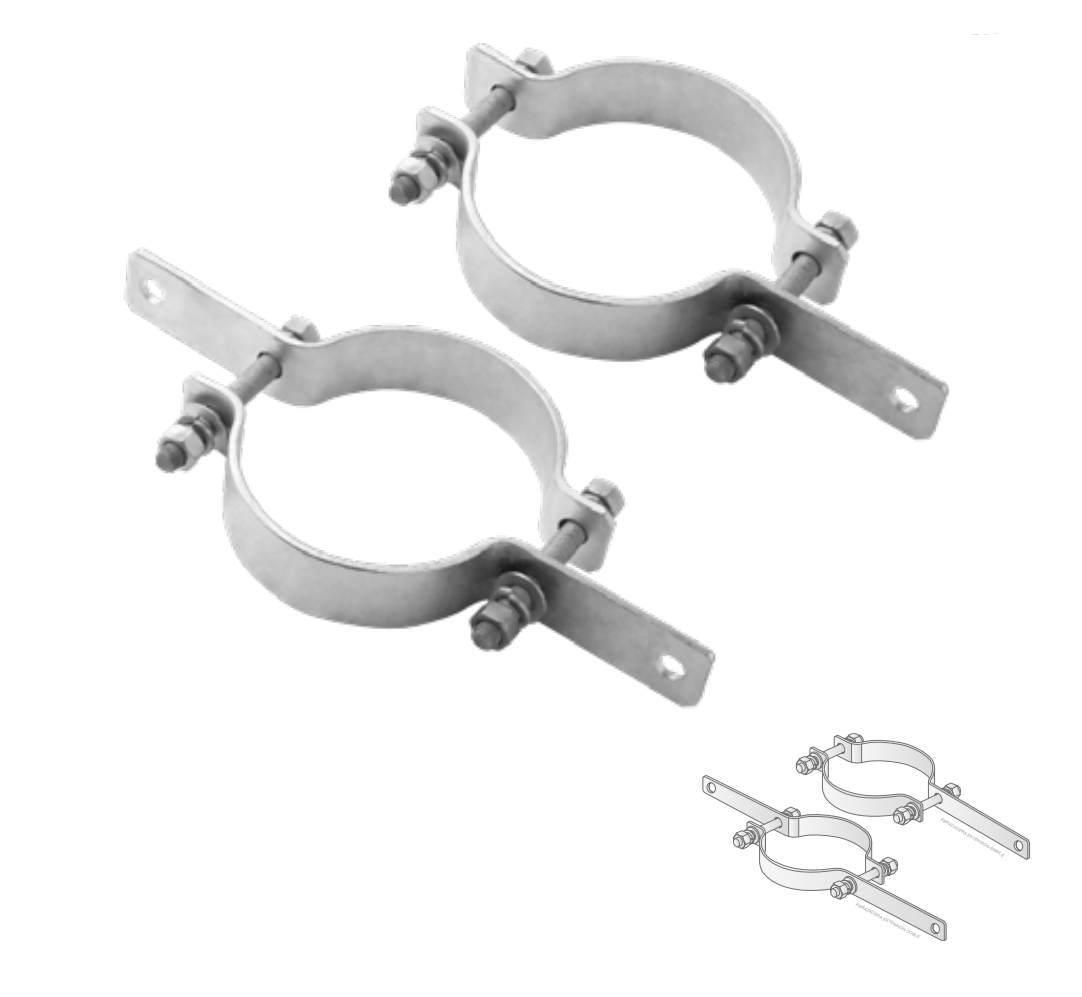
\includegraphics[width=\linewidth]{fotosherrajes/abrazadera de suspension.png}
    \captionof{figure}{\textit{Abrazadera de Suspensión}} % Usa \captionof si no estás en un entorno figure
    \footnotesize
    \raggedright
    \textbf{Nota.} Herraje utilizado para suspender cables o conductores de un soporte.
\end{minipage}%
\hfill% Espacio entre minipáginas
\begin{minipage}[t]{0.48\textwidth} % Minipágina para la Imagen 2
    \centering
    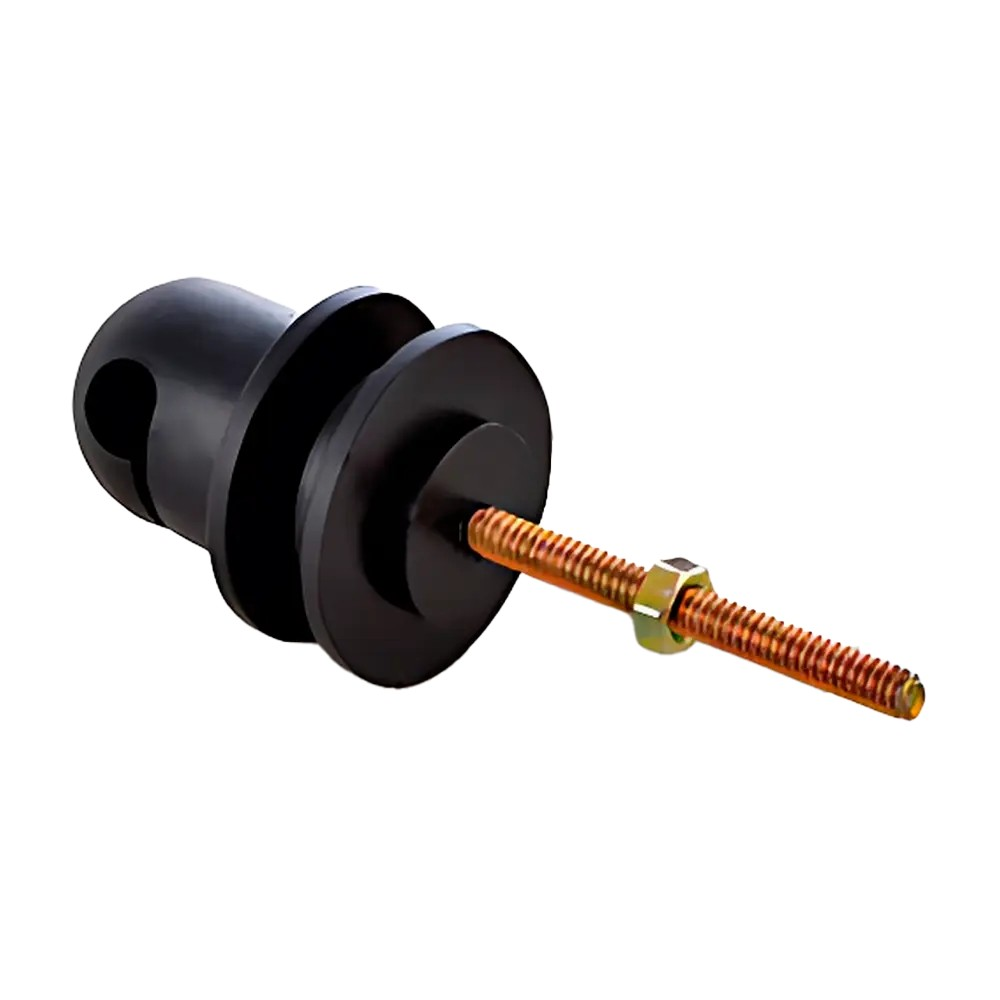
\includegraphics[width=\linewidth]{fotosherrajes/aislador de perno.jpg}
    \captionof{figure}{\textit{Aislador de Perno (Spool Insulator)}}
    \footnotesize
    \raggedright
    \textbf{Nota.} Aislador de bajo voltaje, usualmente montado en un perno para líneas secundarias.
\end{minipage}

\vspace{1cm} % Espacio entre filas

% --- Grupo de Figuras 3 y 4 ---
\noindent % Asegura que no haya sangría al inicio de la línea
\begin{minipage}[t]{0.48\textwidth} % Minipágina para la Imagen 3
    \centering
    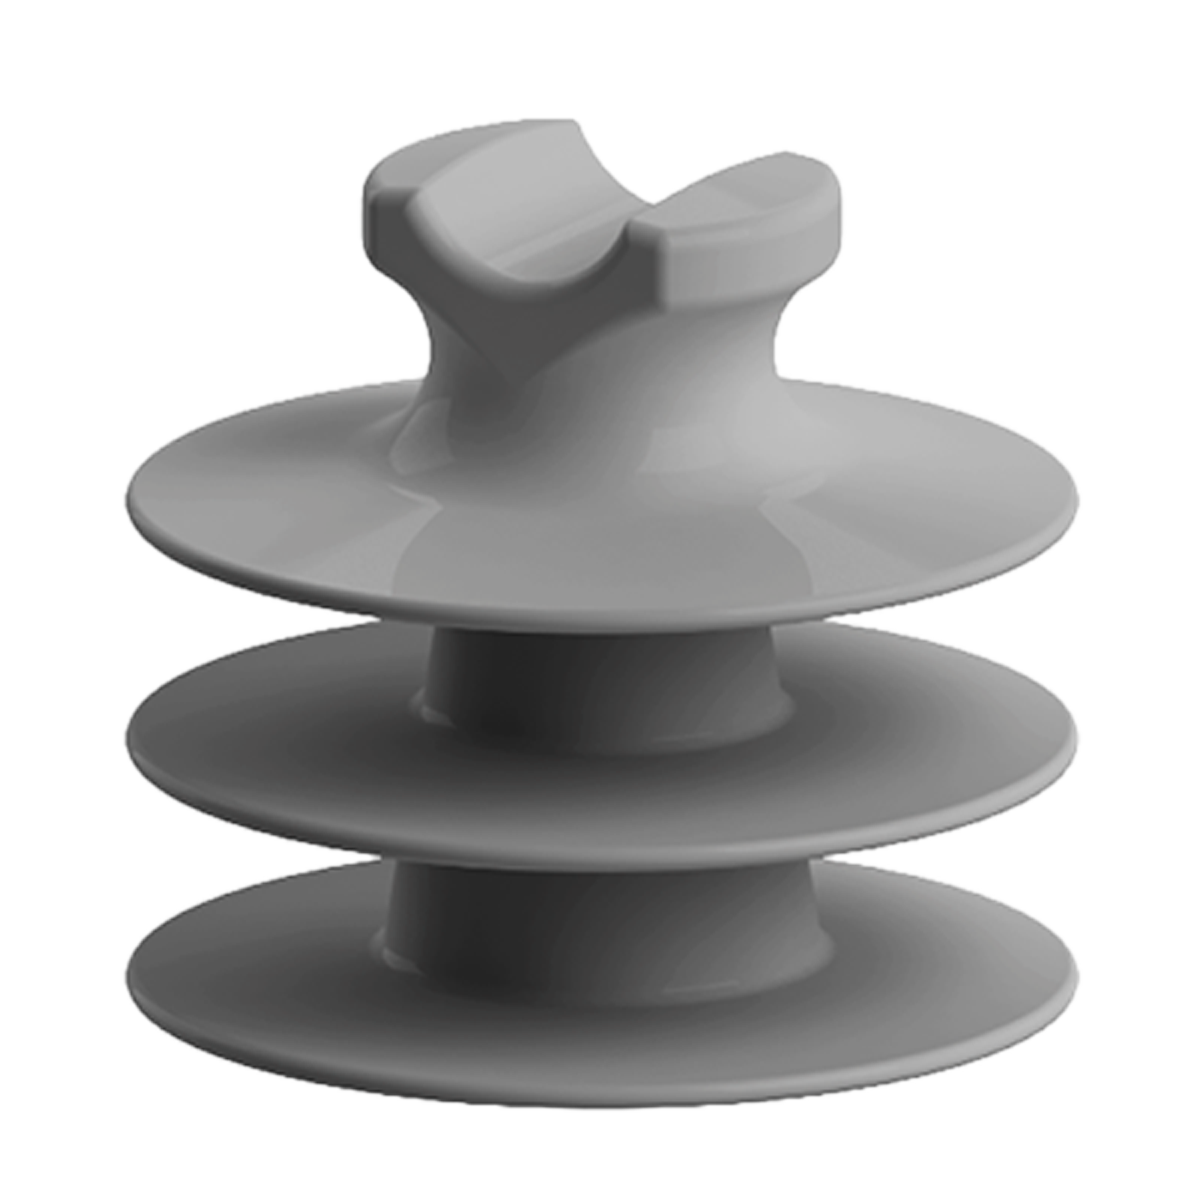
\includegraphics[width=\linewidth]{fotosherrajes/Aislador tipo pin.png}
    \captionof{figure}{\textit{Aislador Eléctrico Tipo Pin}}
    \footnotesize
    \raggedright
    \textbf{Nota.} Aislador montado en un pin o espiga, común en líneas de distribución de voltaje medio.
\end{minipage}%
\hfill% Espacio entre minipáginas
\begin{minipage}[t]{0.48\textwidth} % Minipágina para la Imagen 4
    \centering
    \includegraphics[width=\linewidth]{fotosherrajes/Aislador tipo poste.png}
    \captionof{figure}{\textit{Aislador Eléctrico Tipo Poste}}
    \footnotesize
    \raggedright
    \textbf{Nota.} Aislador sólido utilizado para montar conductores en líneas aéreas.
\end{minipage}

\vspace{1cm} % Espacio entre filas

% --- Grupo de Figuras 5 y 6 ---
\noindent % Asegura que no haya sangría al inicio de la línea
\begin{minipage}[t]{0.48\textwidth} % Minipágina para la Imagen 5
    \centering
    \includegraphics[width=\linewidth]{fotosherrajes/Aislador Tipo Suspensión.png}
    \captionof{figure}{\textit{Aislador Eléctrico Tipo Suspensión}}
    \footnotesize
    \raggedright
    \textbf{Nota.} Cadena de aisladores utilizada para suspender conductores en torres de alta tensión.
\end{minipage}%
\hfill% Espacio entre minipáginas
\begin{minipage}[t]{0.48\textwidth} % Minipágina para la Imagen 6
    \centering
    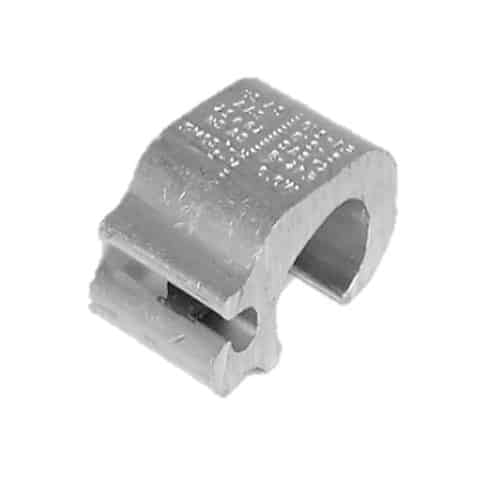
\includegraphics[width=\linewidth]{fotosherrajes/conector de compresion.jpg}
    \captionof{figure}{\textit{Conector de Compresión}}
    \footnotesize
    \raggedright
    \textbf{Nota.} Dispositivo utilizado para unir conductores aplicando presión mecánica (compresión).
\end{minipage}

\vspace{1cm} % Espacio entre filas

% --- Grupo de Figuras 7 y 8 ---
\noindent
\begin{minipage}[t]{0.48\textwidth}
    \centering
    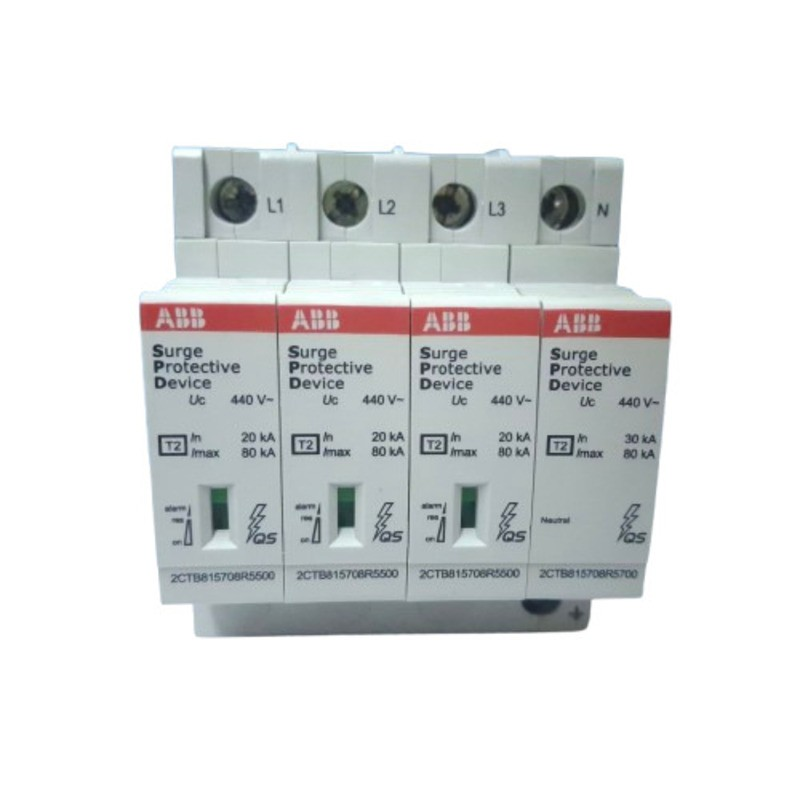
\includegraphics[width=\linewidth]{fotosherrajes/DPS.jpg}
    \captionof{figure}{\textit{Dispositivo de Protección contra Sobretensiones (DPS)}}
    \footnotesize
    \raggedright
    \textbf{Nota.} Equipo diseñado para proteger sistemas eléctricos de picos de voltaje transitorios.
\end{minipage}%
\hfill
\begin{minipage}[t]{0.48\textwidth}
    \centering
    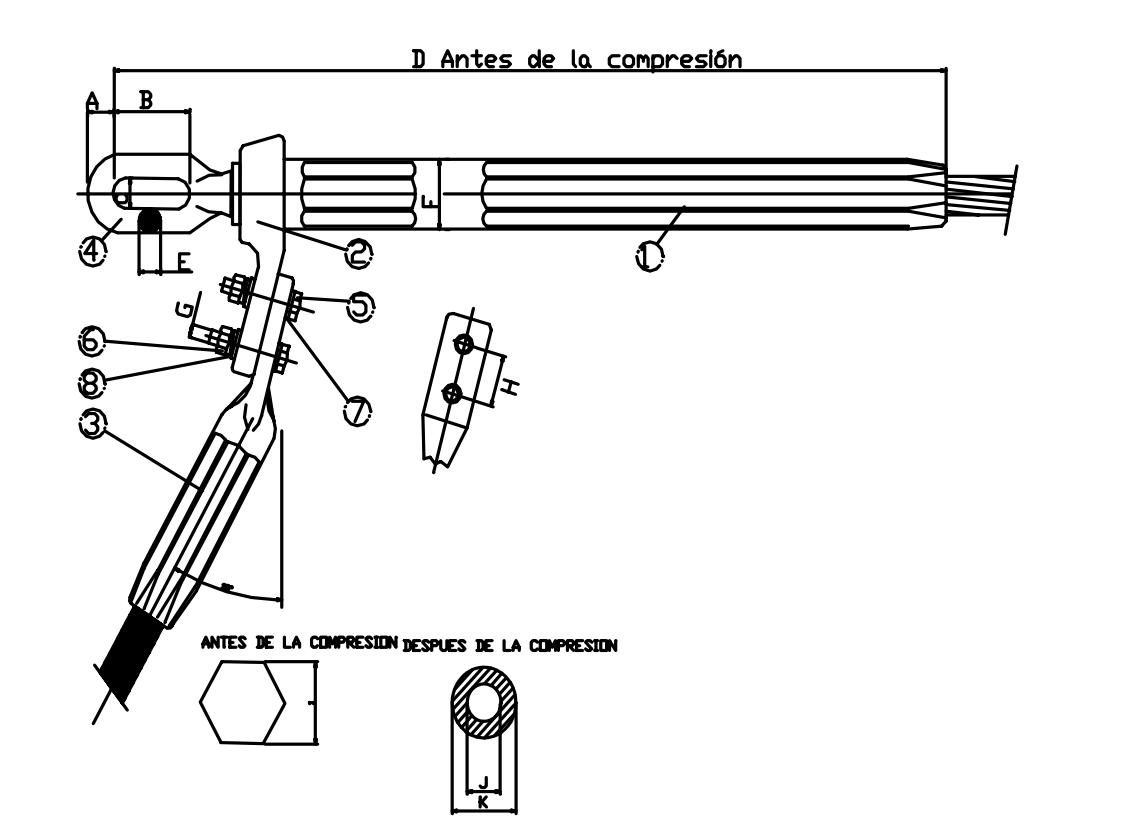
\includegraphics[width=\linewidth]{fotosherrajes/grapa de retencion1.png}
    \captionof{figure}{\textit{Grapa de Retención (Variante 1)}}
    \footnotesize
    \raggedright
    \textbf{Nota.} Herraje utilizado para fijar y retener el conductor en el poste o estructura.
\end{minipage}

\vspace{1cm}

% --- Grupo de Figuras 9 y 10 ---
\noindent
\begin{minipage}[t]{0.48\textwidth}
    \centering
    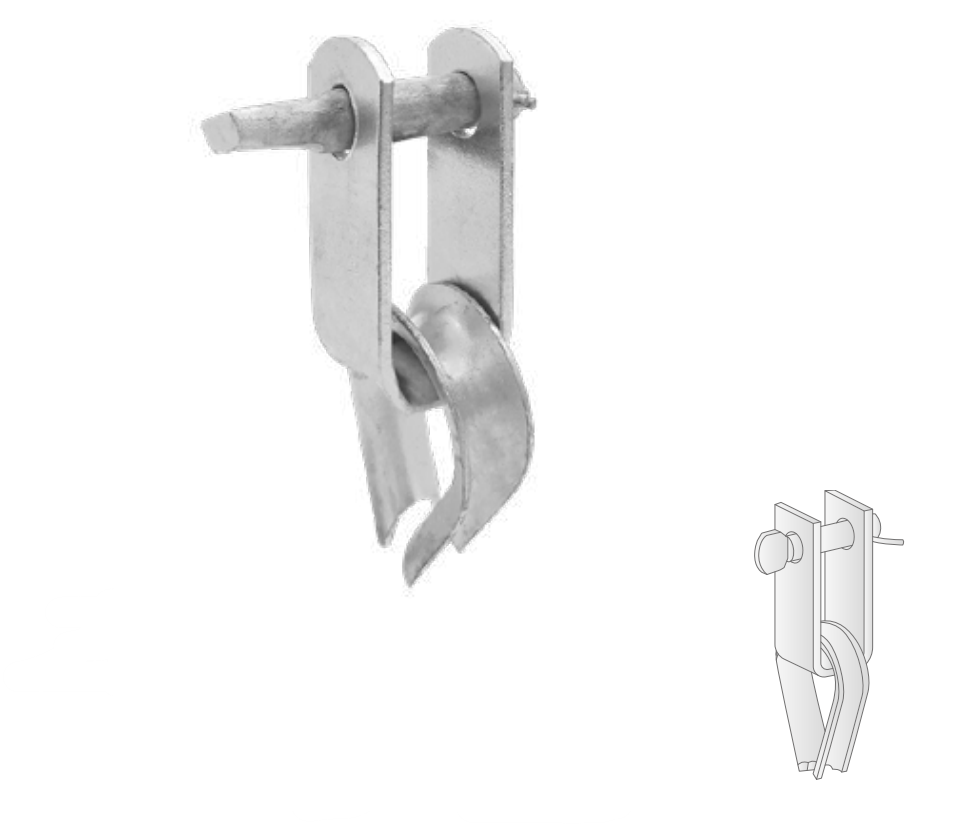
\includegraphics[width=\linewidth]{fotosherrajes/grapa_de_retencion.png}
    \captionof{figure}{\textit{Grapa de Retención (Variante 2)}}
    \footnotesize
    \raggedright
    \textbf{Nota.} Otro tipo de grapa diseñada para aplicaciones de anclaje o retención.
\end{minipage}%
\hfill
\begin{minipage}[t]{0.48\textwidth}
    \centering
    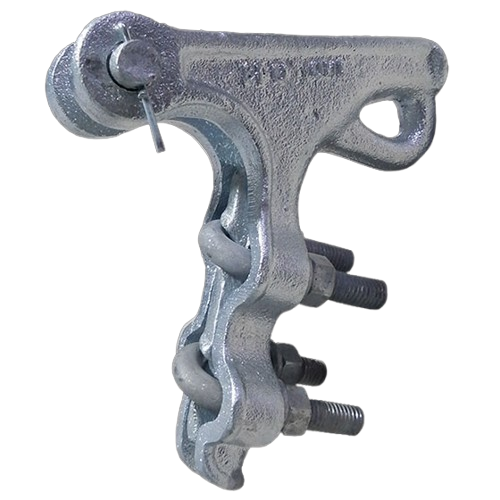
\includegraphics[width=\linewidth]{fotosherrajes/grapas pistola acero.png}
    \captionof{figure}{\textit{Grapas de Acero para Pistola}}
    \footnotesize
    \raggedright
    \textbf{Nota.} Sujetadores de acero utilizados con herramientas de fijación a pólvora o gas.
\end{minipage}

\vspace{1cm}

% --- Grupo de Figuras 11 y 12 ---
\noindent
\begin{minipage}[t]{0.48\textwidth}
    \centering
    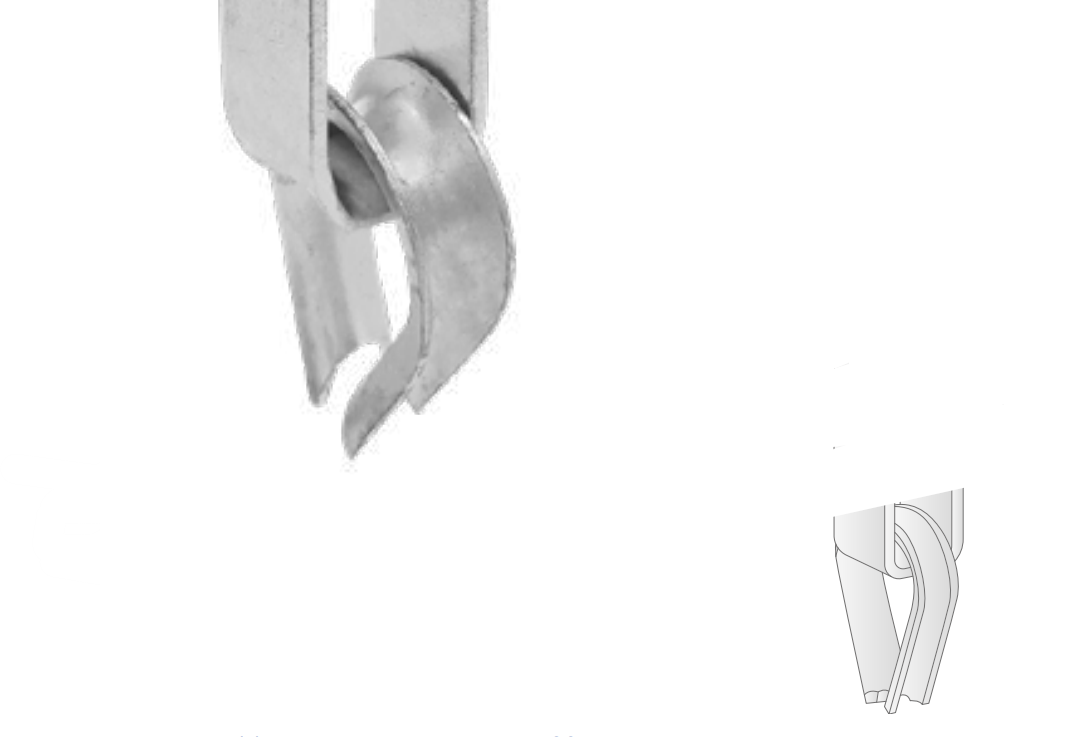
\includegraphics[width=\linewidth]{fotosherrajes/guardacables.png}
    \captionof{figure}{\textit{Guardacables o Dedal}}
    \footnotesize
    \raggedright
    \textbf{Nota.} Pieza que protege un cable o cuerda de fricción y doblamiento excesivo en un lazo.
\end{minipage}%
\hfill
\begin{minipage}[t]{0.48\textwidth}
    \centering
    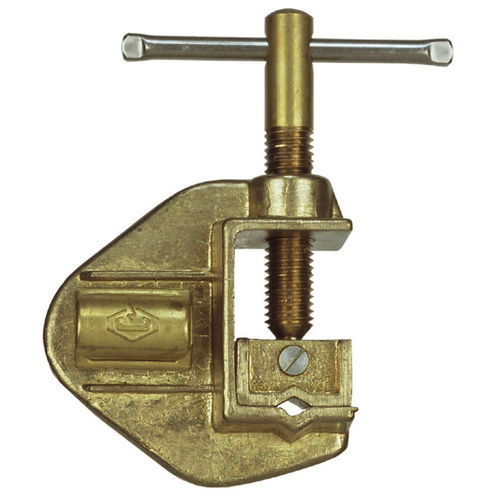
\includegraphics[width=\linewidth]{fotosherrajes/mordaza de conexion a tierra.jpg}
    \captionof{figure}{\textit{Mordaza de Conexión a Tierra}}
    \footnotesize
    \raggedright
    \textbf{Nota.} Conector utilizado para asegurar una conexión eléctrica firme al sistema de puesta a tierra.
\end{minipage}

\vspace{1cm}

% --- Grupo de Figuras 13 y 14 ---
\noindent
\begin{minipage}[t]{0.48\textwidth}
    \centering
    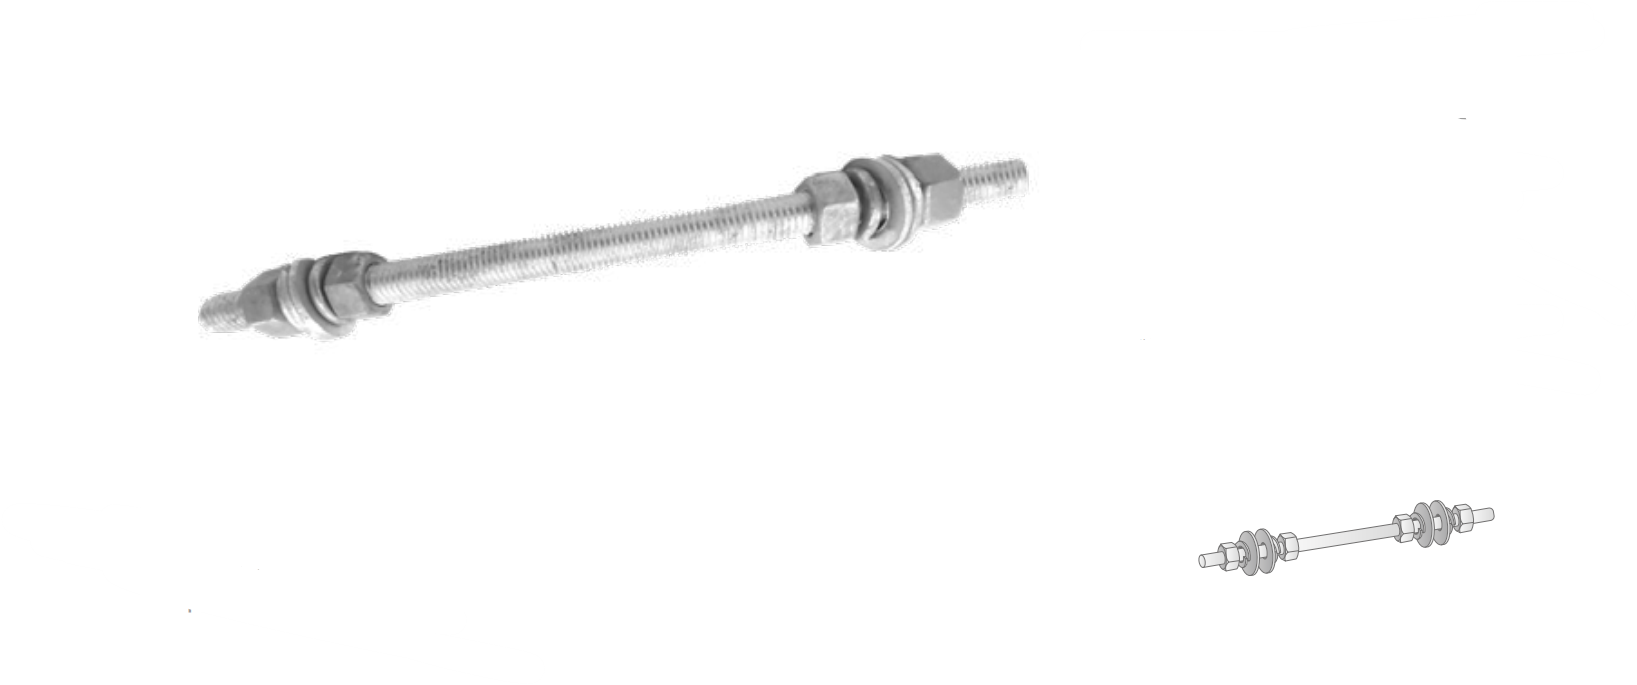
\includegraphics[width=\linewidth]{fotosherrajes/pasadores y arandelas de seguridad.png}
    \captionof{figure}{\textit{Pasadores y Arandelas de Seguridad}}
    \footnotesize
    \raggedright
    \textbf{Nota.} Elementos de fijación utilizados para evitar el aflojamiento o deslizamiento de componentes.
\end{minipage}%
\hfill
\begin{minipage}[t]{0.48\textwidth}
    \centering
    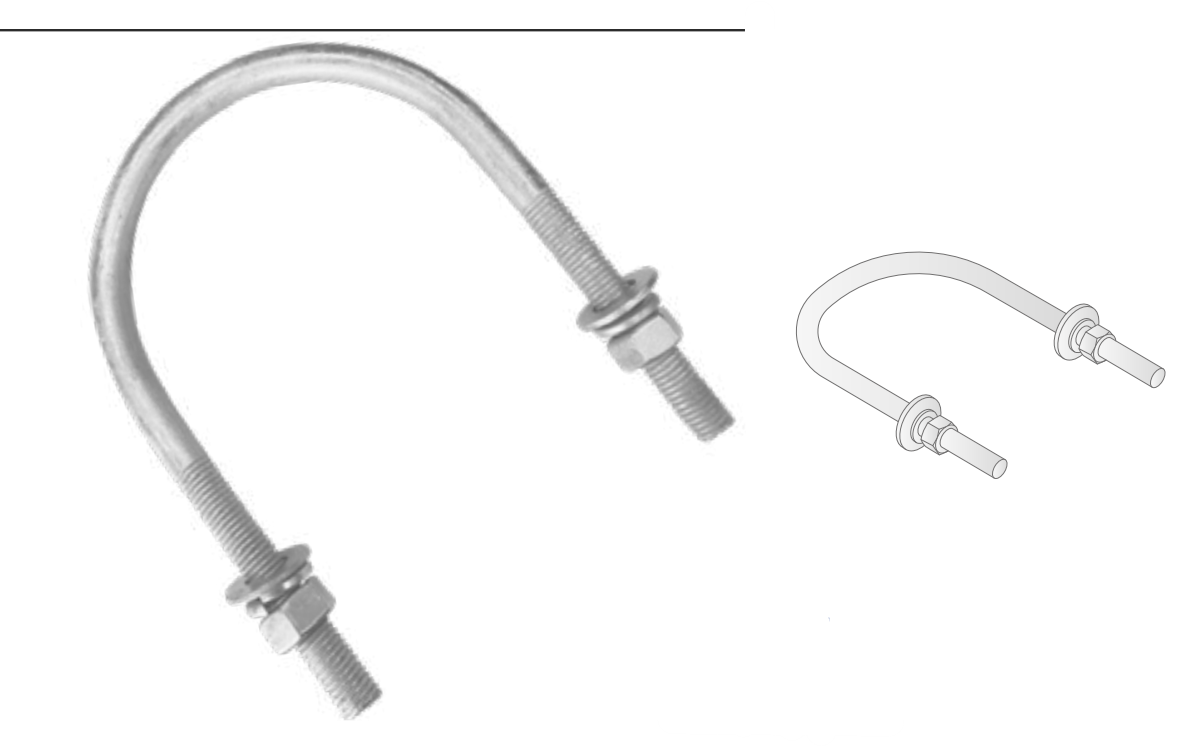
\includegraphics[width=\linewidth]{fotosherrajes/perno de anclaje.png}
    \captionof{figure}{\textit{Perno de Anclaje}}
    \footnotesize
    \raggedright
    \textbf{Nota.} Tornillo o espiga gruesa usada para fijar estructuras a cimientos o soportes.
\end{minipage}

\vspace{1cm}

% --- Grupo de Figuras 15 y 16 ---
\noindent
\begin{minipage}[t]{0.48\textwidth}
    \centering
    \includegraphics[width=\linewidth]{fotosherrajes/perno de ojo.png}
    \captionof{figure}{\textit{Perno de Ojo (Eye Bolt)}}
    \footnotesize
    \raggedright
    \textbf{Nota.} Perno con un lazo en un extremo, utilizado para conectar cables o eslingas.
\end{minipage}%
\hfill
\begin{minipage}[t]{0.48\textwidth}
    \centering
    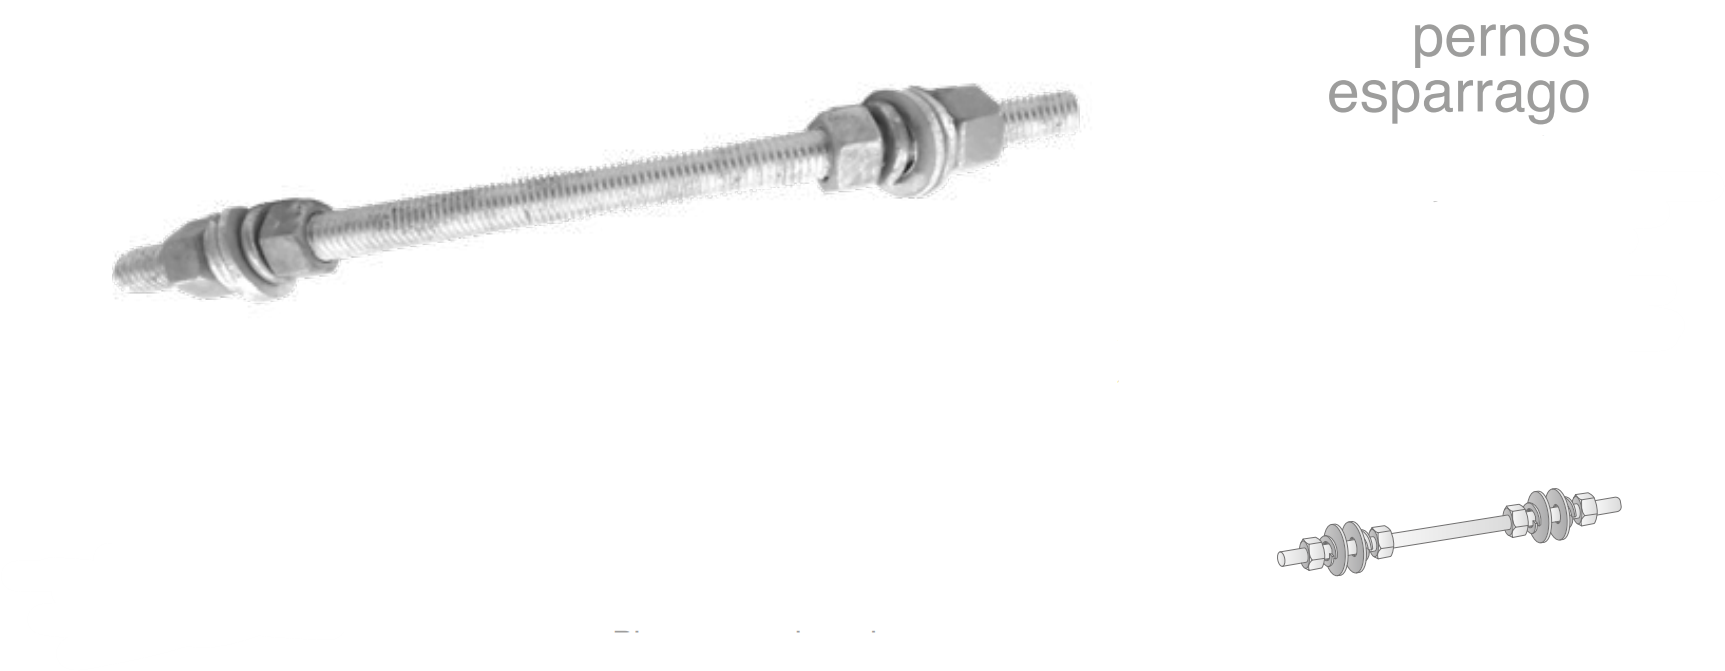
\includegraphics[width=\linewidth]{fotosherrajes/perno de suspension.png}
    \captionof{figure}{\textit{Perno de Suspensión}}
    \footnotesize
    \raggedright
    \textbf{Nota.} Perno especializado para colgar o suspender equipos o componentes.
\end{minipage}

\vspace{1cm}

% --- Grupo de Figuras 17 y 18 ---
\noindent
\begin{minipage}[t]{0.48\textwidth}
    \centering
    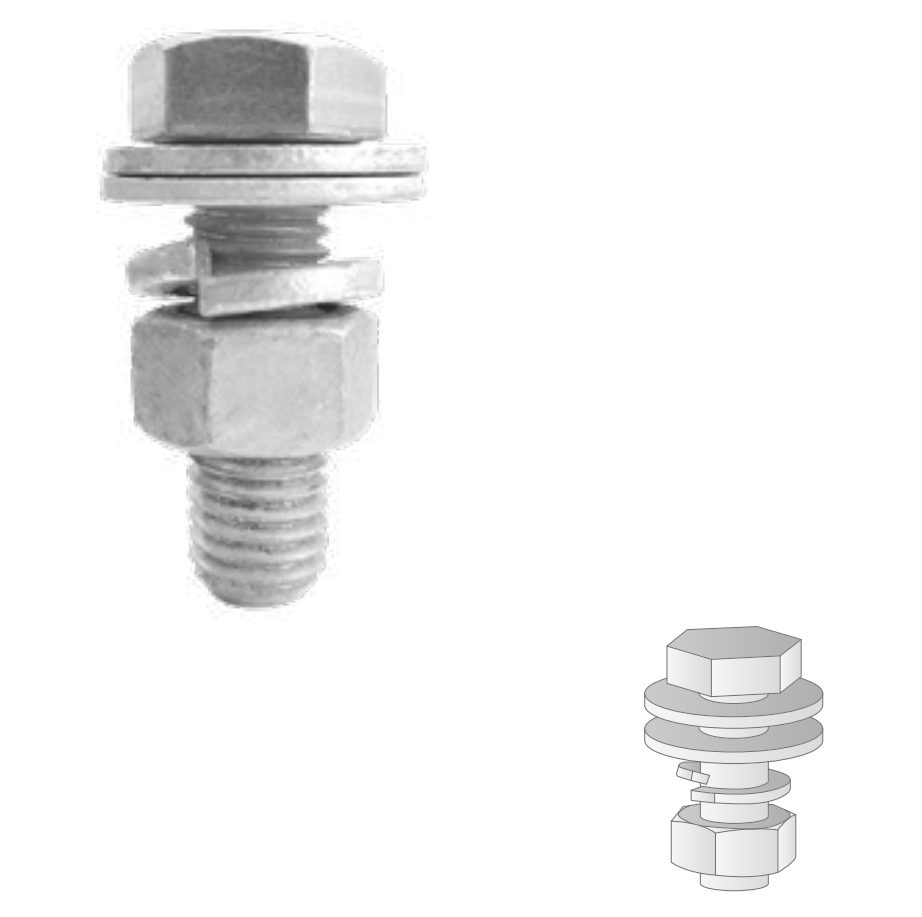
\includegraphics[width=\linewidth]{fotosherrajes/Pernos maquina.png}
    \captionof{figure}{\textit{Pernos Máquina (Tornillos de Máquina)}}
    \footnotesize
    \raggedright
    \textbf{Nota.} Elementos de fijación roscados utilizados en el montaje de piezas metálicas y herrajes.
\end{minipage}%
\hfill
\begin{minipage}[t]{0.48\textwidth}
    \centering
    % Nota: Cambié .webp por .jpg para consistencia según tu lista, pero usa el archivo correcto.
    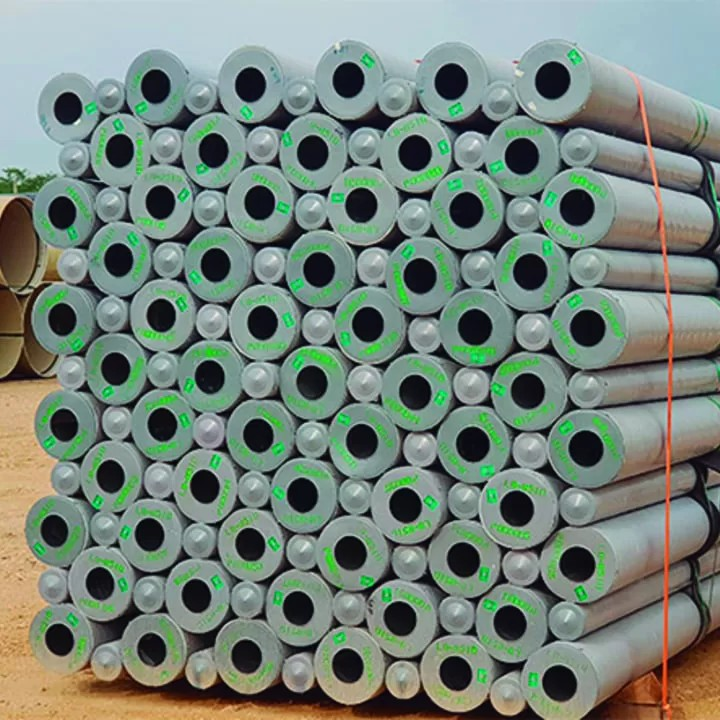
\includegraphics[width=\linewidth]{fotosherrajes/poste fibra de vidrio.jpg}
    \captionof{figure}{\textit{Poste de Fibra de Vidrio}}
    \footnotesize
    \raggedright
    \textbf{Nota.} Poste ligero y resistente a la corrosión, usado en ciertas aplicaciones de líneas eléctricas.
\end{minipage}

\vspace{1cm}

% --- Grupo de Figuras 19 y 20 ---
\noindent
\begin{minipage}[t]{0.48\textwidth}
    \centering
    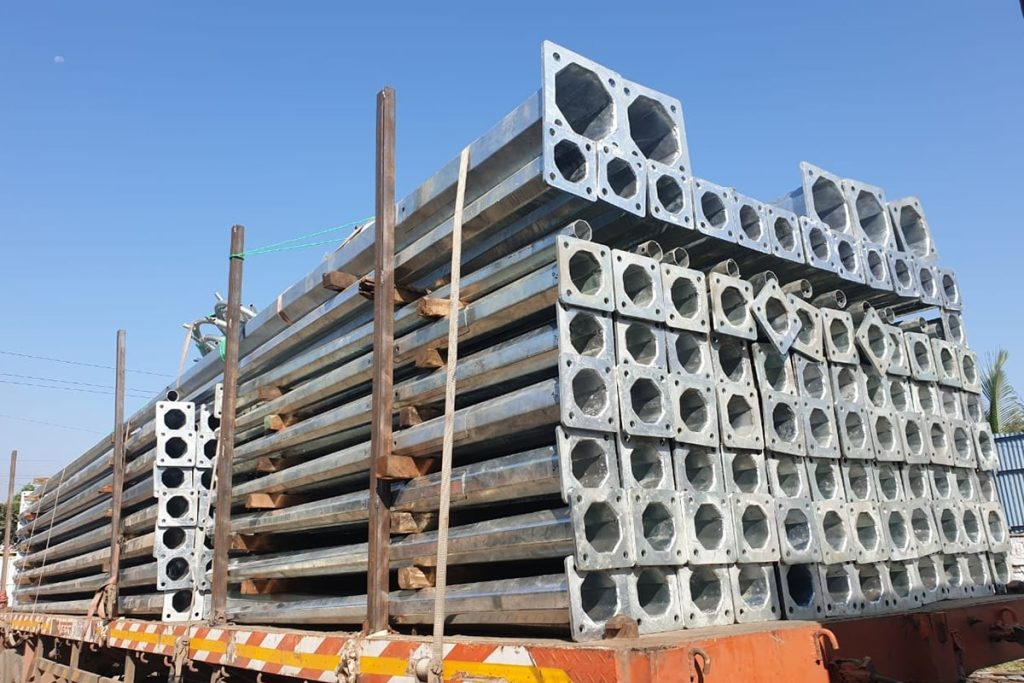
\includegraphics[width=\linewidth]{fotosherrajes/postes acero.jpg}
    \captionof{figure}{\textit{Postes de Acero}}
    \footnotesize
    \raggedright
    \textbf{Nota.} Estructuras metálicas de alta resistencia utilizadas para líneas de transmisión y distribución.
\end{minipage}%
\hfill
\begin{minipage}[t]{0.48\textwidth}
    \centering
    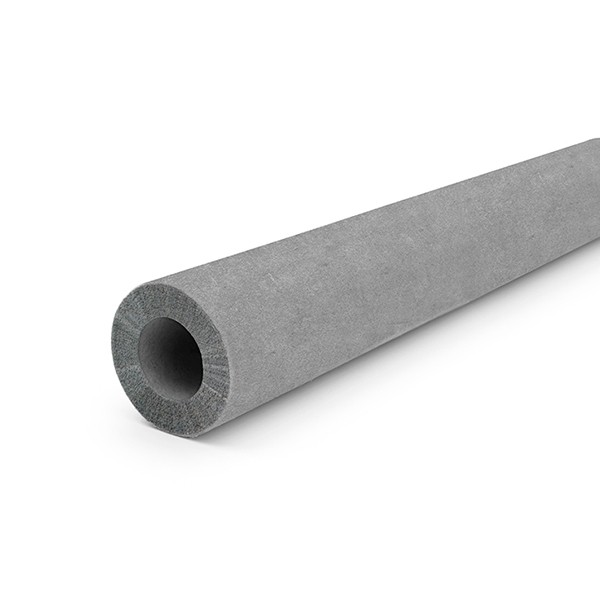
\includegraphics[width=\linewidth]{fotosherrajes/postes concreto.jpg}
    \captionof{figure}{\textit{Postes de Concreto (Hormigón)}}
    \footnotesize
    \raggedright
    \textbf{Nota.} Postes duraderos y de bajo mantenimiento, comunes en redes de distribución urbana.
\end{minipage}

\vspace{1cm}

% --- Grupo de Figuras 21 y 22 ---
\noindent
\begin{minipage}[t]{0.48\textwidth}
    \centering
    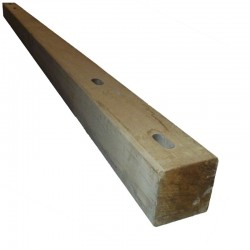
\includegraphics[width=\linewidth]{fotosherrajes/postes maderas.jpg}
    \captionof{figure}{\textit{Postes de Madera}}
    \footnotesize
    \raggedright
    \textbf{Nota.} Postes tradicionales, tratados para resistir la intemperie y el paso del tiempo.
\end{minipage}%
\hfill
\begin{minipage}[t]{0.48\textwidth}
    \centering
    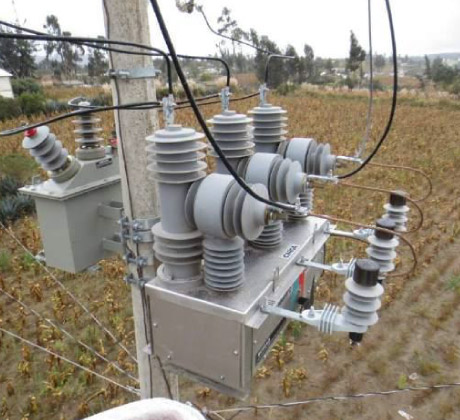
\includegraphics[width=\linewidth]{fotosherrajes/reconectadores.jpg}
    \captionof{figure}{\textit{Reconectadores}}
    \footnotesize
    \raggedright
    \textbf{Nota.} Dispositivos de protección que restauran automáticamente el servicio después de una falla temporal.
\end{minipage}

\vspace{1cm}

% --- Grupo de Figuras 23 y 24 ---
\noindent
\begin{minipage}[t]{0.48\textwidth}
    \centering
    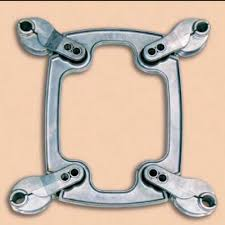
\includegraphics[width=\linewidth]{fotosherrajes/separadores para conductores.jpg}
    \captionof{figure}{\textit{Separadores para Conductores}}
    \footnotesize
    \raggedright
    \textbf{Nota.} Dispositivos para mantener la distancia física y aislamiento entre conductores adyacentes.
\end{minipage}%
\hfill
\begin{minipage}[t]{0.48\textwidth}
    \centering
    \includegraphics[width=\linewidth]{fotosherrajes/tornillos\_de\_seguridad.jpg}
    \captionof{figure}{\textit{Tornillos de Seguridad}}
    \footnotesize
    \raggedright
    \textbf{Nota.} Elementos de fijación diseñados para resistir la manipulación o remoción no autorizada.
\end{minipage}

En resumen, la eficiencia del sistema se logra mediante el diseño optimizado y la gestión de la carga. La seguridad y la fiabilidad son garantizadas por un conjunto coordinado de protecciones, la calidad de los herrajes y una robusta infraestructura estructural y de puesta a tierra.
